\documentclass[12pt]{article} \usepackage{url, graphicx}

% page layout
\setlength{\topmargin}{-0.25in}
\setlength{\textheight}{9.5in}
\setlength{\headheight}{0in}
\setlength{\headsep}{0in}

% problem formatting
\newcommand{\problemname}{Problem}
\newcounter{problem}

% math
\newcommand{\dd}{\mathrm{d}}

% primary units
\newcommand{\rad}{\mathrm{rad}}
\newcommand{\kg}{\mathrm{kg}}
\newcommand{\m}{\mathrm{m}}
\newcommand{\s}{\mathrm{s}}

% secondary units
\renewcommand{\deg}{\mathrm{deg}}
\newcommand{\km}{\mathrm{km}}
\newcommand{\mi}{\mathrm{mi}}
\newcommand{\h}{\mathrm{h}}
\newcommand{\ns}{\mathrm{ns}}
\newcommand{\J}{\mathrm{J}}
\newcommand{\eV}{\mathrm{eV}}
\newcommand{\W}{\mathrm{W}}

% derived units
\newcommand{\mps}{\m\,\s^{-1}}
\newcommand{\mph}{\mi\,\h^{-1}}
\newcommand{\mpss}{\m\,\s^{-2}}

% random stuff
\sloppy\sloppypar\raggedbottom\frenchspacing\thispagestyle{empty}

\begin{document}

\noindent
Name: \rule[-1ex]{0.55\textwidth}{0.1pt}
NetID: \rule[-1ex]{0.2\textwidth}{0.1pt}

\section*{NYU Physics I---Term Exam 4}

\paragraph{\problemname~\theproblem:}\refstepcounter{problem}%
Roughly what is the quality factor $Q$ of this oscillator? (From
Lecture on 2017-10-24.) \\
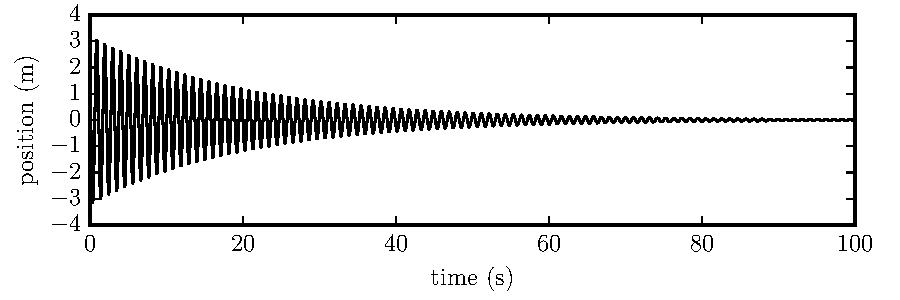
\includegraphics[width=0.66\textwidth]{../py/damped_oscillation.pdf}

\vfill

\paragraph{\problemname~\theproblem:}\refstepcounter{problem}%
You calculated that a pendulum with a period of $2\,\s$ has a length
very close to $1\,\m$. What would be the length of a pendulum with
a period of $8\,\s$? (From Problem Set 7.)

\vfill

\paragraph{\problemname~\theproblem:}\refstepcounter{problem}%
A very thin ladder of length $L$ and mass $M$ leans against a
vertical wall, on a horizontal floor, making an angle of $\theta$ with respect to the
wall. Imagine that there is a large coefficient of friction $\mu$ at the floor such that
the ladder is in static equilibrium, but assume that the wall is effectively
frictionless. Draw a free-body diagram for the ladder, showing all forces acting.
(From Problem Set 8.)

\vfill
~
\clearpage

\paragraph{\problemname~\theproblem:}\refstepcounter{problem}%
In the equation
$$
m\,\frac{\dd^2 x}{\dd t^2} + c\,\frac{\dd x}{\dd t} + k\,x = 0 \quad ,
$$ what are the units of $c$? (From Problem Set 8.)

\vfill

\paragraph{\problemname~\theproblem:}\refstepcounter{problem}%
A mass $m$ attached to a spring of spring constant $k$ is pulled a distance $X$
from it's equilibrium position. What is the potential energy in the
spring? (From worksheet on oscillations.)

\vfill

\paragraph{\problemname~\theproblem:}\refstepcounter{problem}%
If you have a potential of the form
$$
U(x) = A\,x^3 - B\,x + C
$$ where $A$ and $B$ and $C$ are positive constants, find a location $x_0$ where
the force is zero. (From the worksheet on potentials.)

\vfill
~
\end{document}
